% Options for packages loaded elsewhere
\PassOptionsToPackage{unicode}{hyperref}
\PassOptionsToPackage{hyphens}{url}
\PassOptionsToPackage{dvipsnames,svgnames,x11names}{xcolor}
%
\documentclass[
  letterpaper,
  DIV=11,
  numbers=noendperiod]{scrartcl}

\usepackage{amsmath,amssymb}
\usepackage{iftex}
\ifPDFTeX
  \usepackage[T1]{fontenc}
  \usepackage[utf8]{inputenc}
  \usepackage{textcomp} % provide euro and other symbols
\else % if luatex or xetex
  \usepackage{unicode-math}
  \defaultfontfeatures{Scale=MatchLowercase}
  \defaultfontfeatures[\rmfamily]{Ligatures=TeX,Scale=1}
\fi
\usepackage{lmodern}
\ifPDFTeX\else  
    % xetex/luatex font selection
\fi
% Use upquote if available, for straight quotes in verbatim environments
\IfFileExists{upquote.sty}{\usepackage{upquote}}{}
\IfFileExists{microtype.sty}{% use microtype if available
  \usepackage[]{microtype}
  \UseMicrotypeSet[protrusion]{basicmath} % disable protrusion for tt fonts
}{}
\makeatletter
\@ifundefined{KOMAClassName}{% if non-KOMA class
  \IfFileExists{parskip.sty}{%
    \usepackage{parskip}
  }{% else
    \setlength{\parindent}{0pt}
    \setlength{\parskip}{6pt plus 2pt minus 1pt}}
}{% if KOMA class
  \KOMAoptions{parskip=half}}
\makeatother
\usepackage{xcolor}
\setlength{\emergencystretch}{3em} % prevent overfull lines
\setcounter{secnumdepth}{-\maxdimen} % remove section numbering
% Make \paragraph and \subparagraph free-standing
\ifx\paragraph\undefined\else
  \let\oldparagraph\paragraph
  \renewcommand{\paragraph}[1]{\oldparagraph{#1}\mbox{}}
\fi
\ifx\subparagraph\undefined\else
  \let\oldsubparagraph\subparagraph
  \renewcommand{\subparagraph}[1]{\oldsubparagraph{#1}\mbox{}}
\fi


\providecommand{\tightlist}{%
  \setlength{\itemsep}{0pt}\setlength{\parskip}{0pt}}\usepackage{longtable,booktabs,array}
\usepackage{calc} % for calculating minipage widths
% Correct order of tables after \paragraph or \subparagraph
\usepackage{etoolbox}
\makeatletter
\patchcmd\longtable{\par}{\if@noskipsec\mbox{}\fi\par}{}{}
\makeatother
% Allow footnotes in longtable head/foot
\IfFileExists{footnotehyper.sty}{\usepackage{footnotehyper}}{\usepackage{footnote}}
\makesavenoteenv{longtable}
\usepackage{graphicx}
\makeatletter
\def\maxwidth{\ifdim\Gin@nat@width>\linewidth\linewidth\else\Gin@nat@width\fi}
\def\maxheight{\ifdim\Gin@nat@height>\textheight\textheight\else\Gin@nat@height\fi}
\makeatother
% Scale images if necessary, so that they will not overflow the page
% margins by default, and it is still possible to overwrite the defaults
% using explicit options in \includegraphics[width, height, ...]{}
\setkeys{Gin}{width=\maxwidth,height=\maxheight,keepaspectratio}
% Set default figure placement to htbp
\makeatletter
\def\fps@figure{htbp}
\makeatother

\KOMAoption{captions}{tableheading}
\makeatletter
\@ifpackageloaded{caption}{}{\usepackage{caption}}
\AtBeginDocument{%
\ifdefined\contentsname
  \renewcommand*\contentsname{Table of contents}
\else
  \newcommand\contentsname{Table of contents}
\fi
\ifdefined\listfigurename
  \renewcommand*\listfigurename{List of Figures}
\else
  \newcommand\listfigurename{List of Figures}
\fi
\ifdefined\listtablename
  \renewcommand*\listtablename{List of Tables}
\else
  \newcommand\listtablename{List of Tables}
\fi
\ifdefined\figurename
  \renewcommand*\figurename{Figure}
\else
  \newcommand\figurename{Figure}
\fi
\ifdefined\tablename
  \renewcommand*\tablename{Table}
\else
  \newcommand\tablename{Table}
\fi
}
\@ifpackageloaded{float}{}{\usepackage{float}}
\floatstyle{ruled}
\@ifundefined{c@chapter}{\newfloat{codelisting}{h}{lop}}{\newfloat{codelisting}{h}{lop}[chapter]}
\floatname{codelisting}{Listing}
\newcommand*\listoflistings{\listof{codelisting}{List of Listings}}
\makeatother
\makeatletter
\makeatother
\makeatletter
\@ifpackageloaded{caption}{}{\usepackage{caption}}
\@ifpackageloaded{subcaption}{}{\usepackage{subcaption}}
\makeatother
\ifLuaTeX
  \usepackage{selnolig}  % disable illegal ligatures
\fi
\usepackage{bookmark}

\IfFileExists{xurl.sty}{\usepackage{xurl}}{} % add URL line breaks if available
\urlstyle{same} % disable monospaced font for URLs
\hypersetup{
  pdftitle={SI Appendix},
  colorlinks=true,
  linkcolor={blue},
  filecolor={Maroon},
  citecolor={Blue},
  urlcolor={Blue},
  pdfcreator={LaTeX via pandoc}}

\title{SI Appendix}
\author{}
\date{}

\begin{document}
\maketitle

\subsection*{Manuscript Length}\label{manuscript-length}
\addcontentsline{toc}{subsection}{Manuscript Length}

A standard 6-page article is approximately 4,000 words, 50 references,
and 4 medium-size graphical elements (i.e., figures and tables). The
preferred length of articles remains at 6 pages, but PNAS will allow
articles up to a maximum of 12 pages.

\subsubsection*{Digital Figures}\label{digital-figures}
\addcontentsline{toc}{subsubsection}{Digital Figures}

EPS, high-resolution PDF, and PowerPoint are preferred formats for
figures that will be used in the main manuscript. Authors may submit PRC
or U3D files for 3D images; these must be accompanied by 2D
representations in TIFF, EPS, or high-resolution PDF format. Color
images must be in RGB (red, green, blue) mode. Include the font files
for any text.

Images must be provided at final size, preferably 1 column width
(8.7cm). Figures wider than 1 column should be sized to 11.4cm or 17.8cm
wide. Numbers, letters, and symbols should be no smaller than 6 points
(2mm) and no larger than 12 points (6mm) after reduction and must be
consistent.

Figures and tables should be labelled and referenced in the standard way
using the \texttt{\textbackslash{}label\{\}} and
\texttt{\textbackslash{}ref\{\}} commands.

To insert a figure wider than one column, please use the
\texttt{figure*} environment. Figures wider than one column should be
sized to 11.4 cm or 17.8 cm wide. Use \texttt{SCfigure*} environment for
a wide figure with side legends, such as Figure~\ref{fig-side}.

In Quarto, we can do these by setting the \texttt{fig-env} command to
\texttt{figure*} or \texttt{SCfigure*}

\begin{SCfigure*}

\centering{

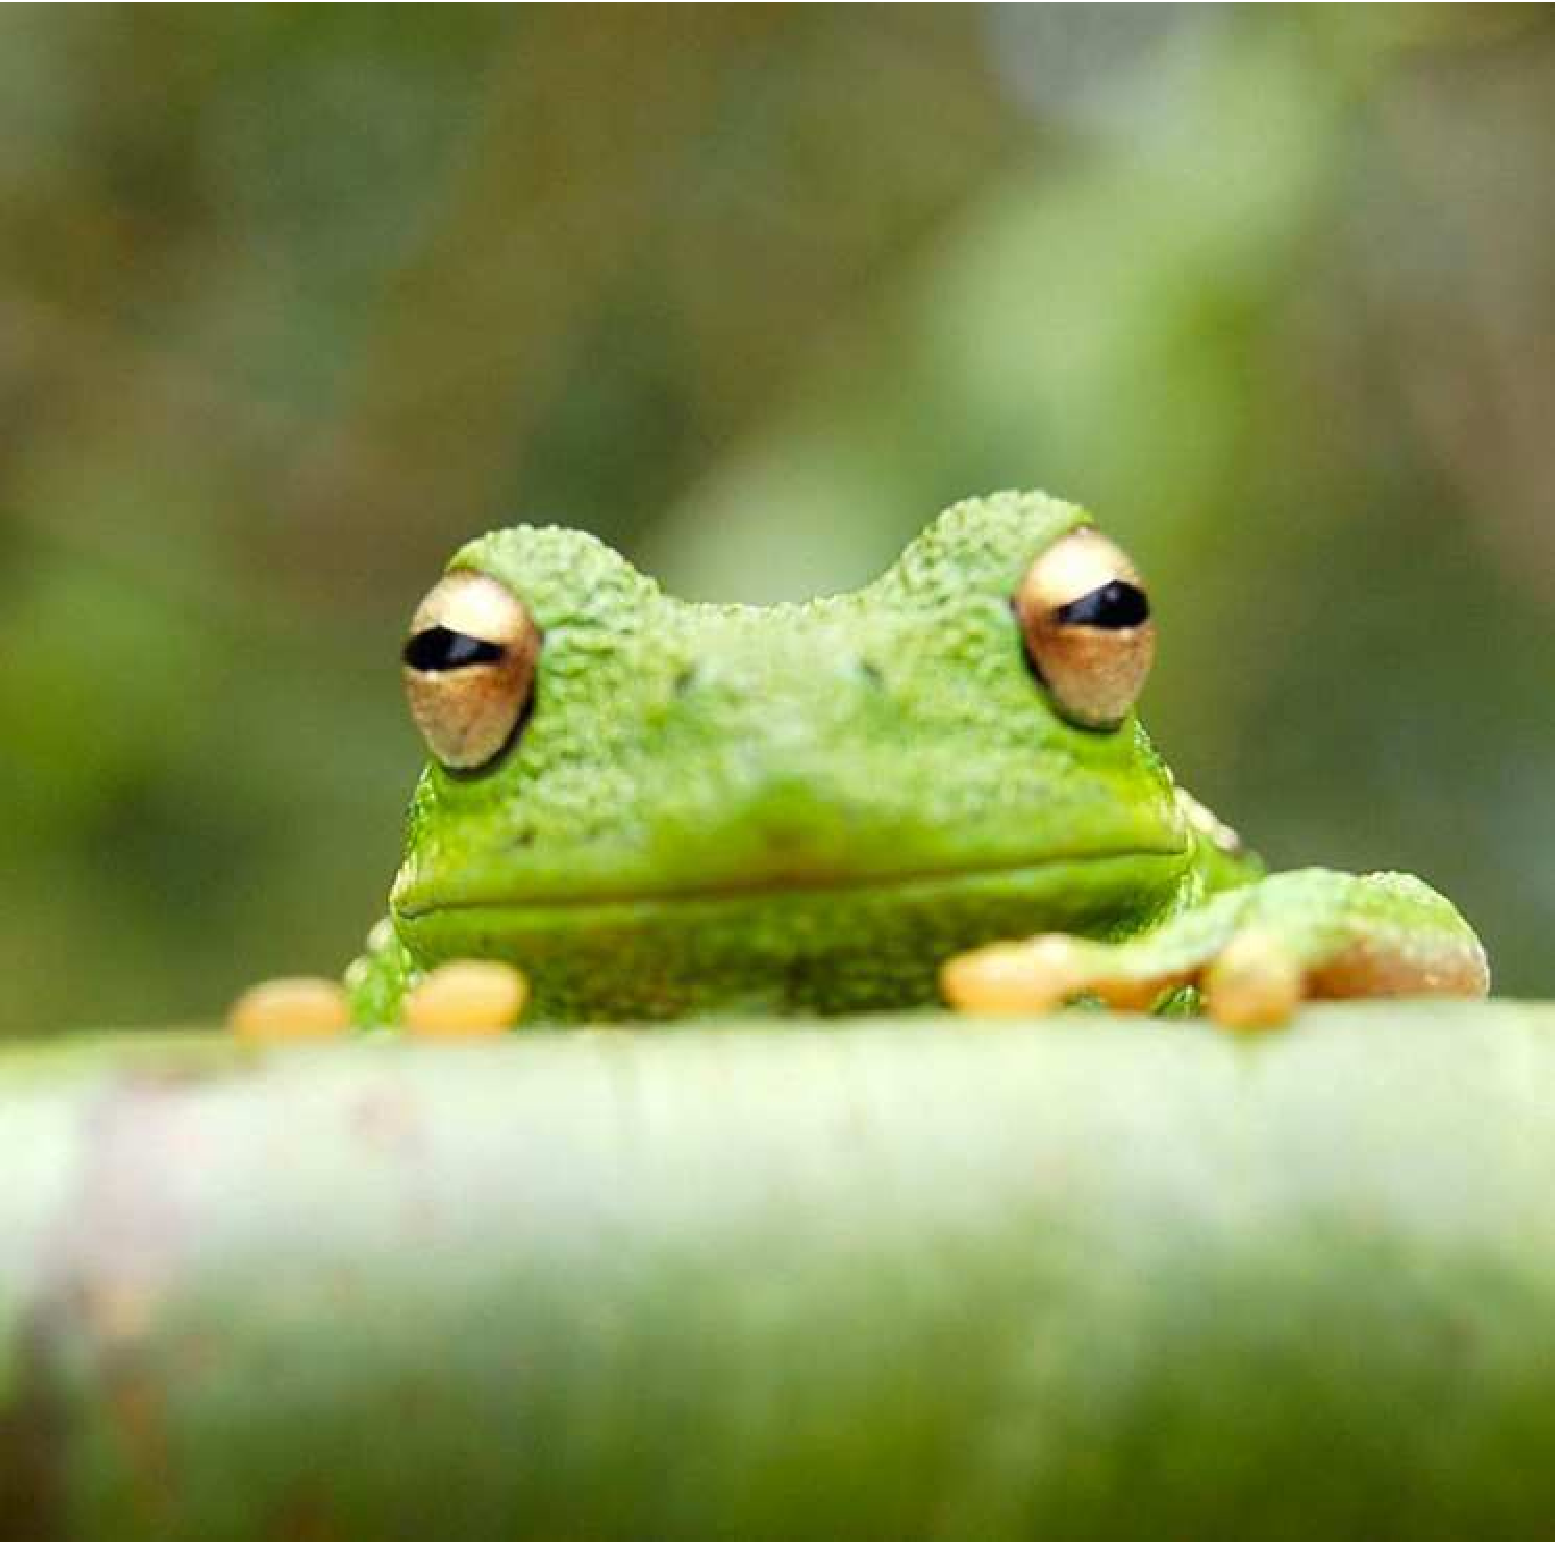
\includegraphics{figs/frog.pdf}

}

\caption{\label{fig-side}This legend would be placed at the side of the
figure, rather than below it.}

\end{SCfigure*}%

\subsection{Supporting Information Appendix
(SI)}\label{supporting-information-appendix-si}

Authors should submit SI as a single separate SI Appendix PDF file,
combining all text, figures, tables, movie legends, and SI references.
SI will be published as provided by the authors; it will not be edited
or composed. Additional details can be found in the
\href{https://www.pnas.org/authors/submitting-your-manuscript\#manuscript-formatting-guidelines}{PNAS
Author Center}. The PNAS Overleaf SI template can be found
\href{https://www.overleaf.com/latex/templates/pnas-template-for-supplementary-information/wqfsfqwyjtsd}{here}.
Refer to the SI Appendix in the manuscript at an appropriate point in
the text. Number supporting figures and tables starting with S1, S2,
etc.Authors who place detailed materials and methods in an SI Appendix
must provide sufficient detail in the main text methods to enable a
reader to follow the logic of the procedures and results and also must
reference the SI methods. If a paper is fundamentally a study of a new
method or technique, then the methods must be described completely in
the main text.

\subsection*{Data Archival}\label{data-archival}
\addcontentsline{toc}{subsection}{Data Archival}

PNAS must be able to archive the data essential to a published article.
Where such archiving is not possible, deposition of data in public
databases, such as GenBank, ArrayExpress, Protein Data Bank, Unidata,
and others outlined in the
\href{https://www.pnas.org/author-center/editorial-and-journal-policies\#materials-and-data-availability}{Information
for Authors}, is acceptable.

\textbf{SI Appendix}

\hfill\break

\textbf{Dataset 1.} SNP-associated effects and standard errors for
green-up estimated using the Gulf genetic subpopulation.

\textbf{Dataset 2.} SNP-associated effects and standard errors for
green-up estimated using the Midwest genetic subpopulation.

\textbf{Dataset 3.} SNP-associated effects and standard errors for
green-up estimated using Both genetic subpopulations.

\textbf{Dataset 4.} SNP-associated effects and standard errors for
flowering estimated using the Gulf genetic subpopulation.

\textbf{Dataset 5.} SNP-associated effects and standard errors for
flowering estimated using the Midwest genetic subpopulation.

\textbf{Dataset 6.} SNP-associated effects and standard errors for
flowering estimated using Both genetic subpopulations.

\textbf{Dataset 7.} Genes within QTL that have functionally validated
roles in flowering in rice.

\textbf{Dataset 8.} Overlap between quantitative trait loci for
flowering measured using an outbred pseudo-F2 mapping population, and
significant mash effect estimates (with a log10Bayes Factor
\textgreater{} 2, or in the 1\% tail of most significant mash results)
found using three overlapping diversity panels. Genes within 20kb with a
functionally validated role in flowering in rice are~ indicated.~

\hfill\break

\textbf{Figure S1.} Variance components analysis of genetic (purple),
genotype by environment (blue), environmental (green), and residual
(yellow) terms in models of green-up time as functions of Julian date or
weather, for the four northern common gardens (North), the three Texas
common gardens (Texas), and for all eight common gardens (All). Dashed
lines indicate the cumulative contribution of G and GxE for flowering as
a function of day of the
year.~\includegraphics{SI_Appendix_files/mediabag/SPDH2Y9HThoK0pUZQxFu.pdf}

\textbf{Figure S2.} Effect patterns exhibited by the major data-driven
matrices for (a,d,e,j,m,n) Gulf, (b,f,g,k,o,p) Midwest, and
(c,h,i,l,q,r) Both subpopulations from Figure 2. (a-i) Green-up date.
(j-r) Flowering date. (a-c,j-l) Single-garden effect representations
(eigenvectors) of the DD\_tPCA data-derived matrices. The percent
variation explained of DD\_tPCA by each eigenvector is shown on the
y-axis. Common gardens are arranged in latitudinal order along the
x-axis. In addition, the first eigenvector corresponds to DD\_PCA\_1,
and second corresponds to DD\_PCA\_2. (d,f,h,m,o,q) The number of SNPs
with significant effects in both conditions that exhibit antagonistic
pleiotropy between that pair of conditions. (e,g,i,n,p,r) Same as
(d,f,h,m,o,q) except for differential sensitivity. Scales for (d,e),
(f,g), (h,i), (m,n), (o,p), and (q,r) are identical and located on the
first panel in alphabetical
order.\includegraphics{SI_Appendix_files/mediabag/JV_8jSfymcCRhEQsEuXD.pdf}

\hfill\break

\hfill\break
\includegraphics{SI_Appendix_files/mediabag/h-CoStrONeN2vAZcGvcr.pdf}

\textbf{Figure S3.} Comparison of mash SNP effects from a diversity
panel and effects from an outbred pseudo-F2 cross. (\textbf{a}) QTL
mapping for four weather-related functions of flowering, and for
green-up date, as indicated by the colors: pink, growing degree days
(GDD) from green-up date to flowering date, yellow, day length change on
the flowering date, green, day length on flowering date; purple,
flowering date; gray, green-up date.Dotted lines indicate
permutation-based significance thresholds for each weather-related
function. Stars indicate QTL with significant enrichment for SNPs in the
1\% mash tail; B, G, and M indicate which subpopulation had enrichment:
B -~ both subpopulations, G - Gulf subpopulation, M -Midwest
subpopulation. Rug plots show genomic locations of SNPs in the 1\% mash
tail for flowering date for each subpopulation. (\textbf{b}) Schematic
comparison of genotypes used for QTL mapping and genotypes used in mash.
(\textbf{c}) Number of mash runs enriched for SNPs in the 1\% mash tail
in the 23 QTL intervals from (\textbf{a}) (dotted red line), compared to
1000 sets of 23 random QTL intervals of the same size
(histogram).\textbf{(d}) SNP effects estimated using mash for SNPs with
the highest Bayes factor for the three QTL with the highest LOD scores
from (\textbf{a}) and enrichment of SNPs in the 1\% mash tail. SNP
genomic position and genetic subpopulation are indicated above each
plot. Common gardens are arranged in latitudinal order. (\textbf{e}) QTL
effect estimates for 23 non-overlapping and partially overlapping QTLs.
Colors indicate which of the four weather-related functions of flowering
for which the QTL was mapped. An additional five QTLs completely
overlapped the QTL displayed; in this case, the QTL with the highest lod
score is shown. Solid vertical lines separate QTLs that are not
overlapping. Stars indicate QTL with significant enrichment for SNPs in
the 1\% mash tail; B, G, and M indicate which subpopulation had
enrichment, as in (\textbf{b}):B -~ both subpopulations, G - Gulf
subpopulation, M -Midwest subpopulation. Common gardens are arranged in
latitudinal order.~

\textbf{Table S1.} Green-up and flowering dates phenotypes linked to
environmental cues.

\begin{longtable}[]{@{}
  >{\raggedright\arraybackslash}p{(\columnwidth - 4\tabcolsep) * \real{0.0659}}
  >{\raggedright\arraybackslash}p{(\columnwidth - 4\tabcolsep) * \real{0.1868}}
  >{\raggedright\arraybackslash}p{(\columnwidth - 4\tabcolsep) * \real{0.7418}}@{}}
\toprule\noalign{}
\endhead
\bottomrule\noalign{}
\endlastfoot
Phenotype & Name & Description \\
green-up & GDD, \textbf{n}d

where `\textbf{n}' is in \{5, 10, 18\} & Correlations in cumulative
growing degree days for the five, ten, or eighteen days prior to
green-up. \\
green-up & Temp Ave, \textbf{n}d

where `\textbf{n}' is in \{5, 10, 18\} & Correlations in average
temperature for the five, ten, or eighteen days prior to green-up. \\
flowering & 50\% green-up & Correlations in green-up. \\
flowering & daylength & Correlations in day length on the day of
flowering. \\
flowering & daylength change (s) & Correlations in the change in
daylength (in seconds) on the day of flowering. \\
flowering & GDD, GR to FL & Correlations in cumulative GDD between
green-up and flowering. \\
flowering & Rainfall, \textbf{n}d sum

where `\textbf{n}' is in \{1, 3, 5\} & Correlations in cumulative
rainfall in the one, three, or five days before flowering, or in the
days between green-up and flowering. \\
\end{longtable}

\hfill\break
\hfill\break

\textbf{Section S1.} Weather-based environmental cues for green-up and
flowering date.

\hfill\break

\begin{verbatim}
We scored green-up and flowering by day of the year, then linked these dates to multiple environmental factors (Table S1). We defined flowering as functions of eight variables: \'flowering date\' (day of the year), cumulative growing degree days (GDD) between green-up and flowering dates (\'flowering GDD\'), day length on the flowering date (\'flowering daylength\'), change in daylength relative to the previous day on the day of flowering (\'flowering daylength change\'), and four measures of cumulative rainfall: cumulative rainfall between green-up and flowering, and in the one day, three days, and five days before flowering. Cumulative GDD was calculated as GDD = GRFLmaxTmean−Tbase,0, where Tmean is the daily average temperature, defined as (Tmax+Tmin)/2, Tbase is the base temperature of 12 °C for switchgrass, Tmax is the maximum daily temperature, Tmin is the minimum daily temperature, GR is green-up date, and FL is flowering date (Kiniry et al. 2005; Behrman et al. 2013).  On a specific day, if Tmean is less than Tbase, the GDD for that day is 0; if Tmean is bigger than Tbase, the GDD for that day is the difference between Tmean and Tbase. We also defined green-up as functions of seven variables: \'green-up date\' (day of the year), cumulative GDD for the five, ten, or eighteen days prior to green-up, and the average air temperature for the five, ten, or eighteen days prior to green-up.

 
\end{verbatim}

\textbf{Section S2.} Hypothesis-based covariance matrix definitions for
mash.

\begin{verbatim}
We generated hypothesis-based covariance matrices derived from correlations in environmental cues in the green-up or flowering date windows for the three subpopulations (Table S1). These covariance matrices were derived from the same set of phenotypes as environmental functions of green-up and flowering, and represent the correlations between genotypes for these phenotypes across our common gardens. For the diagonal of these matrices, we used the coefficient of variation in these phenotypes within the subpopulation at that garden. Code used to generate these matrices can be found at  [git\@github.com](mailto:git@github.com):Alice-MacQueen/pvdiv-phenology-gxe.git/R/Analysis_v0.6_weather_covariance_Uhyp_greenup.Rmd. We used distinct sets of user-specified, hypothesis-based covariance matrices for green-up and flowering, but the same set of matrices for all genetic subgroups. If a hypothesis-based matrix does not capture a common pattern of SNP effects, mash assigns small mixture proportions onto this matrix using maximum likelihood, giving that covariance matrix a low posterior weight summed across all SNP effects, which ultimately causes little to no change in the mash model. Alternatively, SNPs with high mixture proportions on particular environmental covariance matrices and large Bayes factors, which summarize the overall significance of a non-zero effect, represent small genomic intervals with strong evidence for a phenotypic effect correlated with an environmental driver.
\end{verbatim}

\hfill\break

\textbf{Section S3.} Narrow-sense heritability~

\begin{verbatim}
In the diversity panel, we determined narrow-sense heritabilities (h2) for green-up and flowering dates at single gardens using genomic relationship matrices calculated using the van Raden method (VanRaden et al. 2009). Genomic relationship matrices were calculated within each subpopulation (Midwest and Gulf) and for both genetic subpopulations (Both). We used ASReml (VSN International) to specify mixed models of the form:
\end{verbatim}

\textbf{y} = 1 + Zu + e

Var(u) = Gσu2

Var(e) = Iσe2

in which the vector \textbf{y} represents the flowering date or green-up
date values for that garden, Z the design matrix for random effects, u
the whole genome additive genetic effect, and e the residual. Matrix G
is the whole genomic relationship matrix based on all SNPs retained for
subpopulation-specific analyses. I is the rank-y identity matrix.
Phenotypic variance (σp2) is σu2 + σe2. Narrow-sense heritability is
then h2 = (σu2/σp2).

\begin{verbatim}
These models were run for each of the eight gardens, and across all gardens by adding an additional environmental effect of site without an interaction term. This resulted in 54 models: 3 sets of populations (the Gulf, Midwest, and Both subpopulations) for 9 garden sets (all eight gardens separately, and all eight gardens together) and two phenotypes (green-up date and flowering date).
\end{verbatim}

\hfill\break

\textbf{Section S4.} Variance components analysis

\begin{verbatim}
In the diversity panel, to evaluate our environmental cues as genetic triggers of flowering, we defined green-up and flowering for individual genotypes as functions of seven and eight environmental cues, respectively, then used variance components analysis to partition variance attributed to genetic effects (G), genotype by environment interactions (GxE), environmental effects (E), and error for these phenology-related traits using linear mixed models. We used mixed models of the form:
\end{verbatim}

\textbf{y} = 1 + Zuu + Zll + Zulul + e

Var(u) = Gσu2

Var(l) = IσE2

Var(ul) = GσuE2

Var(e) = Iσe2

in which the vector \textbf{y} represents the individual plant
observations of a given trait and Z the design matrices associating
trait observations with random factors. Random factors include u, the
whole genome additive genetic (G) effect, l, the effect of each location
(E), ul, the GxE effect, and e, the residual. Matrix G is the whole
genomic relationship matrix. I are rank-y identity matrices.~

\begin{verbatim}
These models were run for each phenotype as a function of environmental cues. This resulted in 135 models: three sets of populations (the Gulf, Midwest, and Both subpopulations) for three garden sets (All, North, and Texas gardens) and 15 phenotypes (seven green-up functions, and eight flowering functions).
\end{verbatim}

\hfill\break

\textbf{Section S5.} Multivariate adaptive shrinkage

\begin{verbatim}
To evaluate the prevalence and kinds of covariance patterns of SNP effects across our eight common gardens, we used multivariate adaptive shrinkage (mash) on SNP effect estimates from the diversity panel (Urbut et al. 2019). Mash is a statistical method that allows estimation and comparison of many effects jointly across many different conditions; it improves on previous methods by allowing arbitrary correlations in effect sizes among conditions. To this end, mash allows the user to include hypothesis-based covariance matrices, specifies some \'canonical\' covariance matrices with simple patterns of effects, and also generates \'data-driven\' covariance matrices from patterns of effects in the data. Then, mash assigns mixture proportions for each SNP onto each provided covariance matrix using maximum likelihood. Finally, mash uses Bayes\' theorem to shrink effects for each SNP towards the set of covariance matrices in accordance to their mixture proportions. For example, a SNP affecting flowering may have a high mixture proportion, or weight, on a covariance matrix created from a specific environmental cue. In that case, we can infer that the effect of that SNP on flowering is caused by a response to or interaction with that environmental cue. These user-specified and data-driven covariance matrices are an important advantage mash offers for studying patterns of GxE: the user-specified covariance matrices allow hypothesis testing of specific environmental drivers for each SNP, while the data-driven covariance matrices allow exploration of additional unexplained patterns of covariation. 

We first conducted univariate GWAS at each common garden for green-up and flowering date, then analyzed the allelic effects for the top 19K unlinked SNPs per univariate GWAS using mash, as in Lovell et al. (2021). To allow for the possibility that different subpopulations had different strengths of connection between our phenotypes and genotypes (Korte and Farlow 2013), we conducted three sets of genetic analyses: on Gulf and Midwest genotypes separately, and on both subpopulations together (hereafter \'Both\' subpopulations). Only SNPs with ≤ 20% missing data and minor allele frequencies \> 0.05 were used in univariate GWAS, resulting in 8.8 million SNPs retained for the Midwest subpopulation, 10.3 million SNPs retained for the Gulf subpopulation, and 12.3 million SNPs retained for Both subpopulations. Then, we created a set of \'random\' markers to account for correlation in effects using a set of 19K relatively unlinked (r2 \< 0.2) markers. Next, we created a set of \'strong\' markers by selecting 19K SNPs with the largest -log10(p-value) in any condition in the univariate GWAS, out of all markers unlinked at (r2 \< 0.2), which represented the SNP with the strongest effect in the 19K LD blocks with the largest univariate effects. We used the \'pvdiv_standard_run()\' function of the switchgrassGWAS R package (https://github.com/Alice-MacQueen/switchgrassGWAS) to conduct GWAS on genotypes from the Midwest, Gulf, and Both subpopulations, used the \'pvdiv_bigsnp2mashr()\' function to convert univariate GWAS output to the matrices of effects and standard errors needed for mash, then used the \'mash_standard_run()\' function to conduct mash, again specifying distinct sets of hypothesis-based covariance matrices for green-up and flowering, but the same set of matrices for all genetic subgroups. 
\end{verbatim}

\hfill\break

\textbf{Section S6.} Outbred pseudo-F2 mapping population and
Quantitative Trait Locus mapping

\begin{verbatim}
To confirm candidate genomic regions and patterns of allelic effects found in the diversity panel, we analyzed flowering in an outbred pseudo-F2 cross between four individuals, two Midwest and two Gulf individuals. The formation of this mapping population has been described previously (Milano, Lowry, and Juenger 2016). The parents of this cross were DAC, an early flowering Midwest individual, VS16, a late flowering Midwest individual, AP13, an early flowering Gulf individual, and WBC, a late flowering Gulf individual. We made F1 crosses of the two early flowering genotypes, AP13xDAC, and the two late flowering genotypes, WBCxVS16. We then clonally propagated and planted the four parents, the two F1 genotypes (AP13xDAC, and VS16xWBC), and 801 F2 genotypes at eight field sites in May-July of 2015. To be directly comparable to the diversity panel data, only 2019 phenology data from the pseudo-F2 cross from the same eight common garden sites were used here. 

Details on the genetic map construction, map polishing and fine-scale reordering can be accessed on <https://datadryad.org/stash/dataset/doi:10.5061/dryad.ghx3ffbjv>. QTL mapping was conducted with R/qtl2 (Broman et al. 2019). We performed a genome scan with a linear mixed model that accounts for the relationships among individuals and for environmental covariates (i.e., field sites). The full model can be expressed as: phenotype = µ + QTL + E + QTLxE + kinship + e, where µ is the population mean, QTL is the marker genetic effect, E is the environmental effects (here, common garden), QTLxE is the interaction between marker genetic and environmental effects, kinship corresponds to the background polygenic variation, and e is the error term. The genome scan was accomplished with the \'scan1\' function. The statistical significance of the genome scan was established by performing a stratified (i.e., stratifying on common garden) permutation test (n=1000) using \'scan1perm\' function. The estimated QTL effect was obtained using \'scan1coef\' function in R/qtl2. 
\end{verbatim}



\end{document}
